\documentclass{article}
\usepackage[paperwidth=7.6cm,paperheight=12.8cm,margin=0pt]{geometry}
\usepackage{fontspec,tikz}
\usepackage[table]{xcolor}
\usetikzlibrary{arrows.meta}
\IfFontExistsTF{Helvetica Neue}
  {\setmainfont{Helvetica Neue}\setsansfont{Helvetica Neue}}
  {\IfFontExistsTF{Arial}{\setmainfont{Arial}\setsansfont{Arial}}{}}
\definecolor{navy}{HTML}{315E75}
\definecolor{teal}{HTML}{2E766E}
\definecolor{amber}{HTML}{A17431}
\definecolor{ink}{HTML}{2B3A42}
\definecolor{mute}{HTML}{7A8C94}
\definecolor{lightblue}{HTML}{EAF3F7}
\definecolor{lightteal}{HTML}{EDF6F2}
\definecolor{lightamber}{HTML}{FAF3E5}
\definecolor{lightrow}{HTML}{F7FAFB}
\definecolor{hairline}{HTML}{BDD0D8}
\pagestyle{empty}
\begin{document}
\noindent\hspace*{7mm}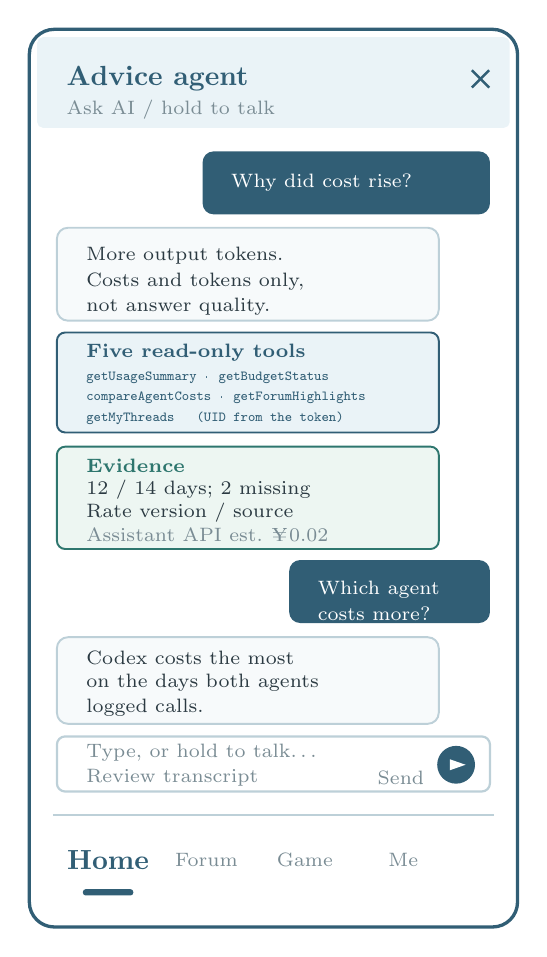
\begin{tikzpicture}[every node/.style={text=ink}]
\draw[draw=navy,line width=1.2pt,rounded corners=9pt] (0,0) rectangle (6.2,11.4);
% panel header
\fill[lightblue,rounded corners=2pt] (.10,10.15) rectangle (6.10,11.30);
\node[anchor=west,font=\bfseries,text=navy] at (.35,10.78) {Advice agent};
\node[anchor=west,font=\scriptsize,text=mute] at (.35,10.38) {Ask AI / hold to talk};
\draw[draw=navy,line width=.9pt] (5.62,10.66) -- (5.84,10.88);
\draw[draw=navy,line width=.9pt] (5.62,10.88) -- (5.84,10.66);
% user question (right)
\fill[navy,rounded corners=4pt] (2.20,9.05) rectangle (5.85,9.85);
\node[anchor=west,font=\scriptsize,text=white] at (2.44,9.45) {Why did cost rise?};
% assistant answer (left)
\fill[lightrow,rounded corners=4pt] (.35,7.70) rectangle (5.20,8.88);
\draw[draw=hairline,line width=.7pt,rounded corners=4pt] (.35,7.70) rectangle (5.20,8.88);
\node[anchor=west,font=\scriptsize] at (.60,8.52) {More output tokens.};
\node[anchor=west,font=\scriptsize] at (.60,8.20) {Costs and tokens only,};
\node[anchor=west,font=\scriptsize] at (.60,7.88) {not answer quality.};
% the five read-only tools the service may call
\fill[lightblue,rounded corners=3pt] (.35,6.28) rectangle (5.20,7.55);
\draw[draw=navy,line width=.7pt,rounded corners=3pt] (.35,6.28) rectangle (5.20,7.55);
\node[anchor=west,font=\scriptsize\bfseries,text=navy] at (.60,7.30) {Five read-only tools};
\node[anchor=west,font=\fontsize{5}{6}\selectfont\ttfamily,text=navy] at (.60,6.98)
  {getUsageSummary · getBudgetStatus};
\node[anchor=west,font=\fontsize{5}{6}\selectfont\ttfamily,text=navy] at (.60,6.72)
  {compareAgentCosts · getForumHighlights};
\node[anchor=west,font=\fontsize{5}{6}\selectfont\ttfamily,text=navy] at (.60,6.46)
  {getMyThreads \quad (UID from the token)};
% evidence box
\fill[lightteal,rounded corners=3pt] (.35,4.80) rectangle (5.20,6.10);
\draw[draw=teal,line width=.7pt,rounded corners=3pt] (.35,4.80) rectangle (5.20,6.10);
\node[anchor=west,font=\scriptsize\bfseries,text=teal] at (.60,5.86) {Evidence};
\node[anchor=west,font=\scriptsize] at (.60,5.56) {12 / 14 days; 2 missing};
\node[anchor=west,font=\scriptsize] at (.60,5.26) {Rate version / source};
\node[anchor=west,font=\scriptsize,text=mute] at (.60,4.98) {Assistant API est. ¥0.02};
% second user question
\fill[navy,rounded corners=4pt] (3.30,3.86) rectangle (5.85,4.66);
\node[anchor=west,font=\scriptsize,text=white] at (3.54,4.28) {Which agent};
\node[anchor=west,font=\scriptsize,text=white] at (3.54,3.98) {costs more?};
% second assistant answer
\fill[lightrow,rounded corners=4pt] (.35,2.58) rectangle (5.20,3.68);
\draw[draw=hairline,line width=.7pt,rounded corners=4pt] (.35,2.58) rectangle (5.20,3.68);
\node[anchor=west,font=\scriptsize] at (.60,3.42) {Codex costs the most};
\node[anchor=west,font=\scriptsize] at (.60,3.10) {on the days both agents};
\node[anchor=west,font=\scriptsize] at (.60,2.78) {logged calls.};
% input bar — typing stays available even if the microphone is denied
\fill[white,rounded corners=3pt] (.35,1.72) rectangle (5.85,2.42);
\draw[draw=hairline,line width=.8pt,rounded corners=3pt] (.35,1.72) rectangle (5.85,2.42);
\node[anchor=west,font=\scriptsize,text=mute] at (.60,2.22) {Type, or hold to talk…};
\node[anchor=west,font=\scriptsize,text=mute] at (.60,1.90) {Review transcript};
\node[anchor=west,font=\scriptsize,text=mute] at (4.30,1.90) {Send};
\fill[navy] (5.42,2.06) circle (.24);
\fill[white] (5.34,1.99) -- (5.54,2.06) -- (5.34,2.13) -- cycle;
% bottom navigation — the assistant is entered from Home, which is the landing
% tab, so the highlight sits there.
\draw[hairline,line width=.6pt] (.30,1.42) -- (5.90,1.42);
\node[font=\bfseries,text=navy] at (1.00,.85) {Home};
\node[font=\scriptsize,text=mute] at (2.25,.85) {Forum};
\node[font=\scriptsize,text=mute] at (3.50,.85) {Game};
\node[font=\scriptsize,text=mute] at (4.75,.85) {Me};
\fill[navy,rounded corners=1pt] (.68,.40) rectangle (1.32,.48);
\end{tikzpicture}
\end{document}
